% Pixel DAQ System

The intention of this section it to give an overview of
the CMS pixel DAQ system. For more details the reader
can follow the references given in the text. But the
introduction given here should be sufficient to understand
the main goals of the pixel software.

\subsection{Overview of DAQ components}

The CMS pixel DAQ system consists of a number of 
components as illustrated in Fig.~\ref{fig:daqcomponents}.
This figure is specific to the FPix detector, but the
modification for the BPix are minor and not really 
relevant to the discussion here unless otherwise 
mentioned. Starting from the detector itself we have the the
Read Out Chip (ROC)~\cite{ROC} and the token bit manager 
(TBM)~\cite{TBM}. Some properties of the ROC are described 
below as needed to understand the calibrations. The
ROC reads out 4,160 pixels and the TBM coordinates
the communication with a group of 8 to 24 ROCs.
The TBM is electrically connected to the portcard via
extension cables $\approx 2$ feet in length.

The portcard receives and sends optical signals to the
FrontEnd Controller (FEC) and FrontEnd Driver (FED)
respectively. The FEC is used to program the TBM 
and ROCs and the data read out from the detector is
send to the FED to be digitized. The portcard is the
home of several discrete components. We have the 
Digital Optic Hybrid (DOH) that receives data from
the FEC and the Analog Optic Hybrid (AOH) that 
transmits data to the FED. On the portcard we
have in addition the (t)PLL, Delay25, and gatekeeper
chips. 

Of particular interest is the Delay25 chip. The communication
to the portcard via the DOH is done at 40MHz on a serial
line. We have a clock line and the data line (and return clock
and return data). In order to have this communication
working the timing between the clock and data lines must
be right. The purpose of the Delay25 chip is to adjust
delays to make this communication work. The setting of the
parameters on the Delay25 chip as well as the other components
on the portcard is done using the I2C protocol from the
CCU. The CCU is again controlled from a Tracker FEC (TkFEC).

\begin{figure}[h]
\begin{center}
 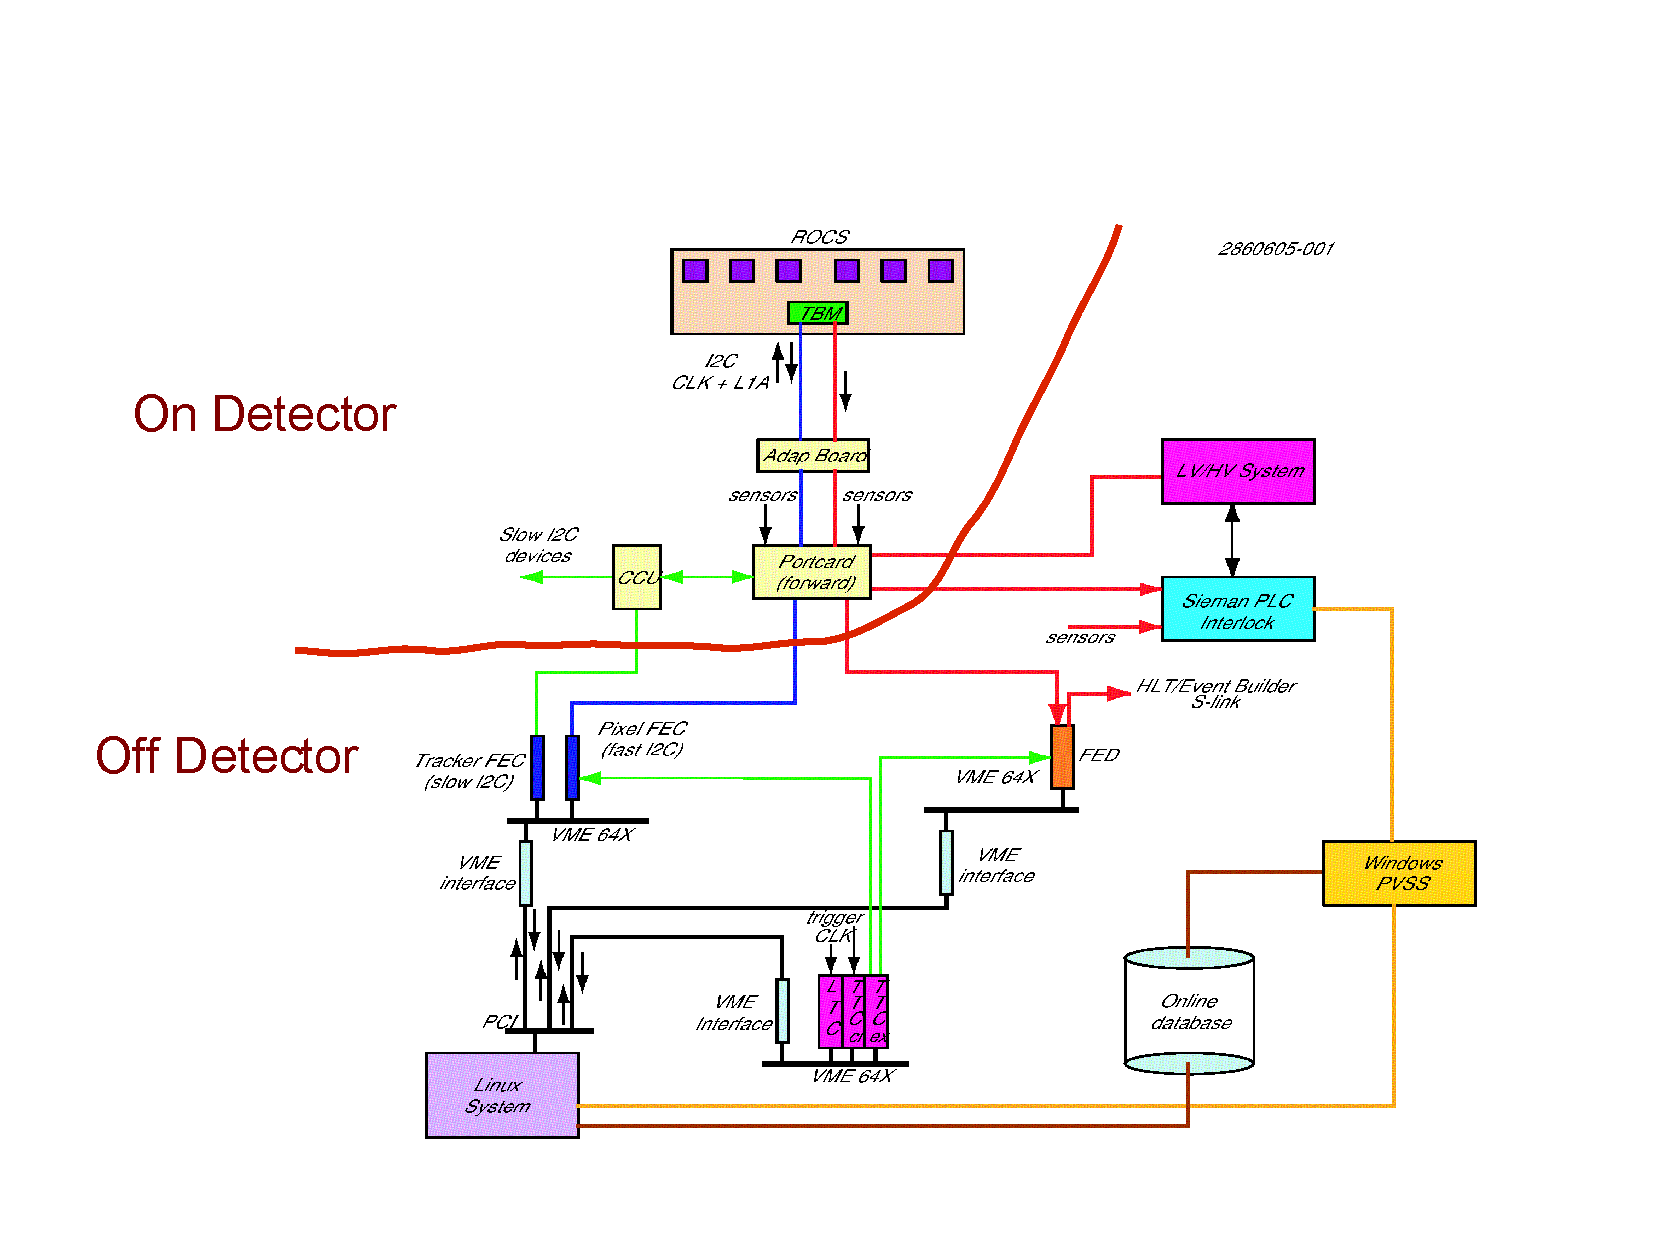
\includegraphics[width=0.99\textwidth]{2860506-001}
\end{center}
\caption{The main components in the CMS pixel DAQ system. }
\label{fig:daqcomponents}
\end{figure}

\clearpage

\subsubsection{The Read Out Chip}

Each Read Out Chip (ROC)~\cite{ROC}, ilustrated in Fig.~\ref{fig:ROC} collates data from 52 $\times$ 80 = 4,160 pixels 
and contains about 1.3 million transistors in all.
It amplifies and zero suppresses data using 4 trim bits
that specify a threshold for every pixel. The chip buffers hit data
until the trigger decision arrives. It is developed at PSI and manufactured by IBM.

\begin{figure}[h]
\begin{center}
 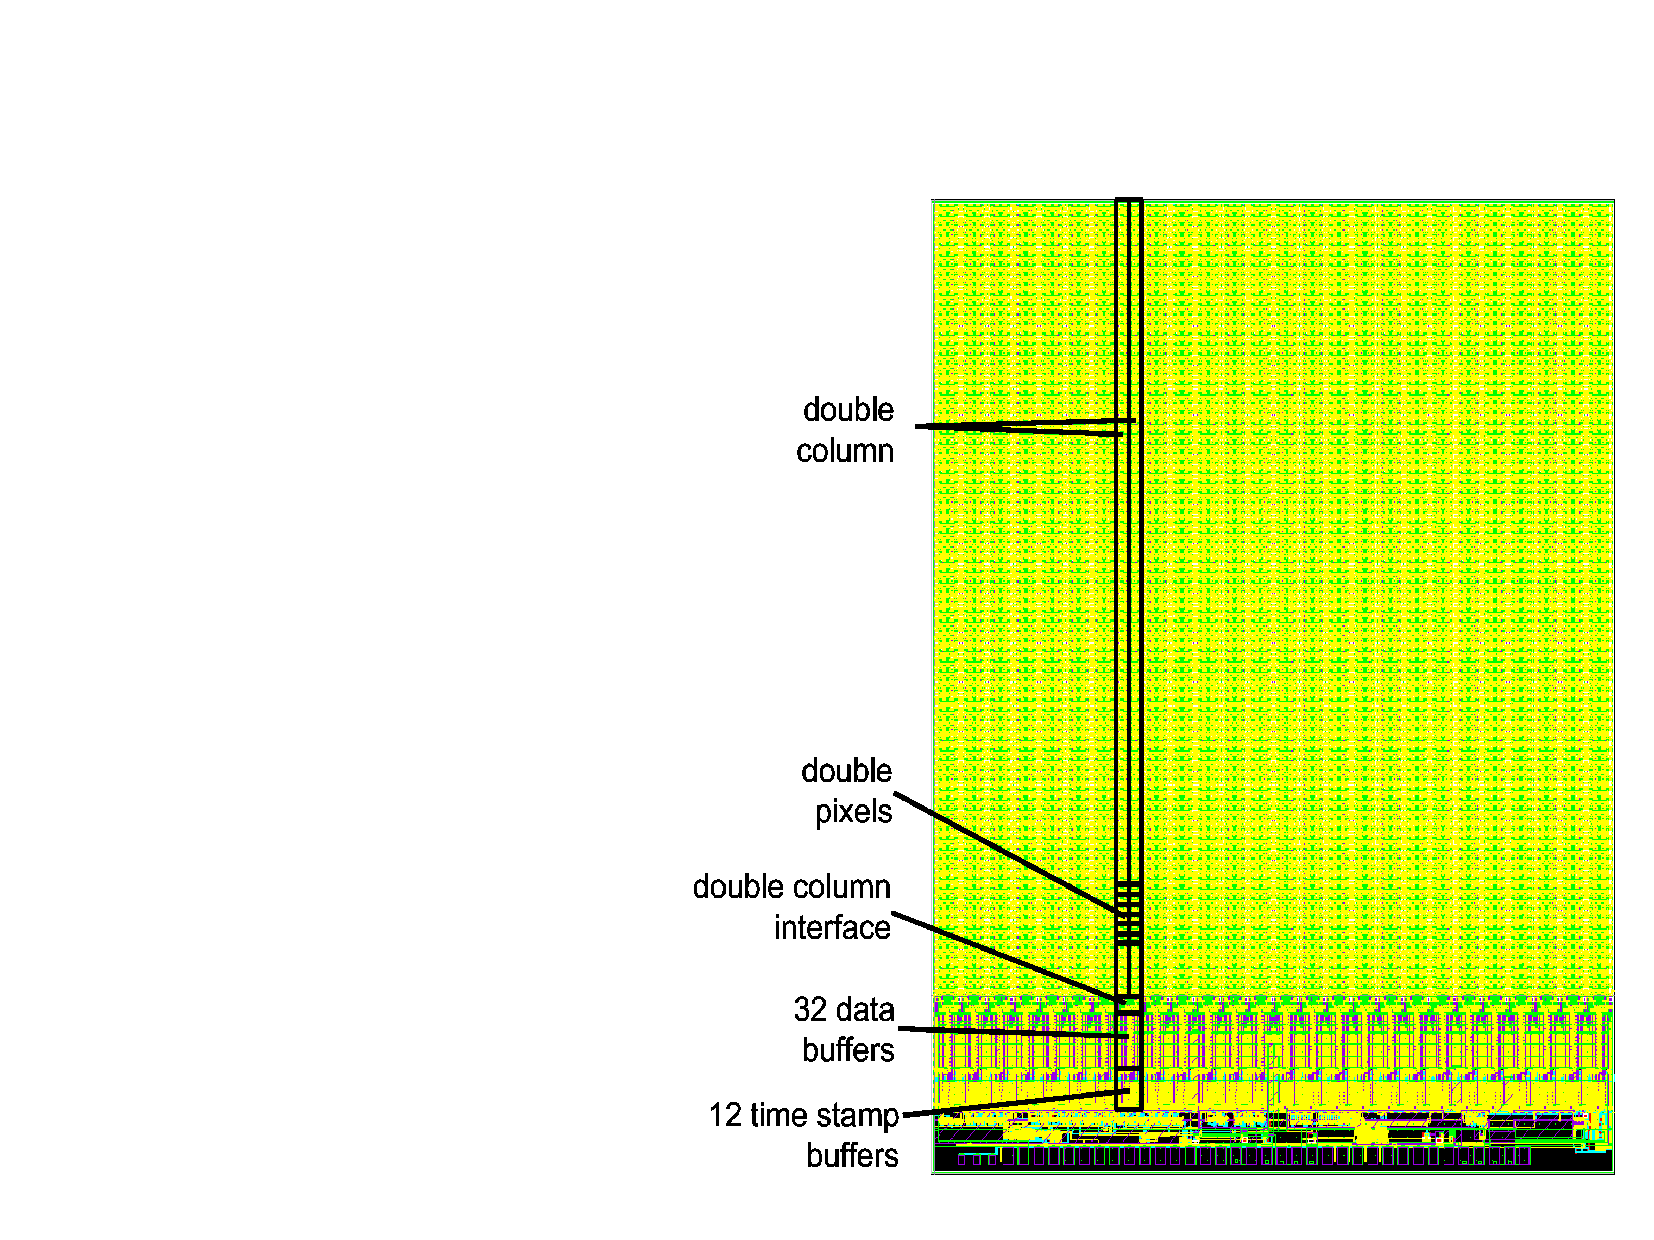
\includegraphics[width=0.45\textwidth]{ROC.pdf}
\end{center}
\caption{The Read Out Chip of the CMS Pixel Detector.}
\label{fig:ROC}
\end{figure}

\clearpage

\subsubsection{The Token Bit Manager}

A Token Bit Manager (TBM) controls groups of 8 to 24 ROCs.
It distributes the clock and trigger signals.
It serializes analog readout using a token bit 
passed from ROC to ROC. It is physically mounted next to the ROCs.
The TBM is developed at Rutgers.

\begin{figure}[h]
\begin{center}
 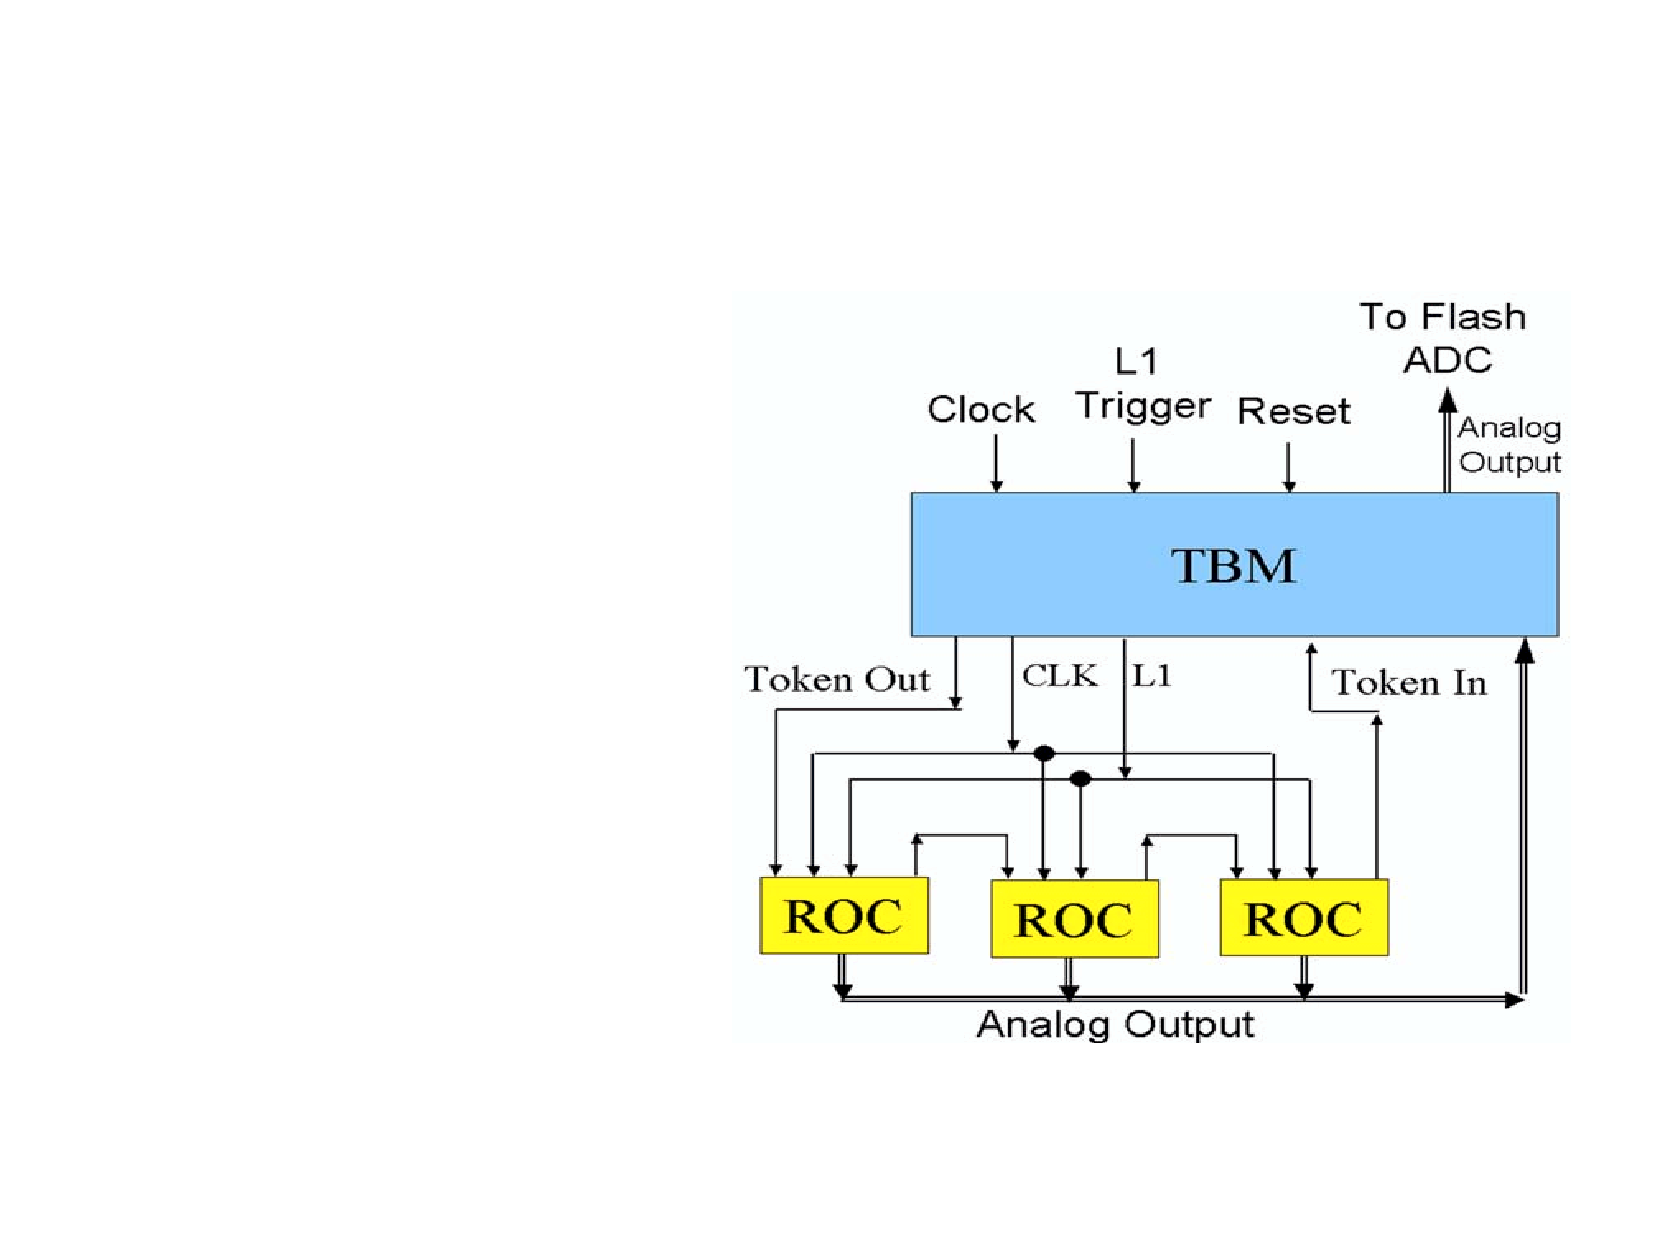
\includegraphics[width=0.45\textwidth]{TBM.pdf}
\end{center}
\caption{A schematic of how the Token Bit Manager reads out data from the ROCs.}
\label{fig:TBM}
\end{figure}

\clearpage

\subsubsection{The Pixel FED}

The Pixel Front End Driver (FED) is a VME module
with 36 optical inputs. It sits in the counting room and receives the analog output
of the ROCs via an optical fiber from the center of the CMS detector.
In order for the FED to decode and digitize this data, it has to have address levels 
well calibrated, and this is one of the several tasks performed by the Pixel Online Software.
Internal timings of the FED also have to be calibrated within errors of a few nanoseconds,
and this is also accomplished using the POS. The output of the FED
is dispatched, in a binary format readable to the entire CMS experiment, via an S-Link.

\begin{figure}[h]
\begin{center}
 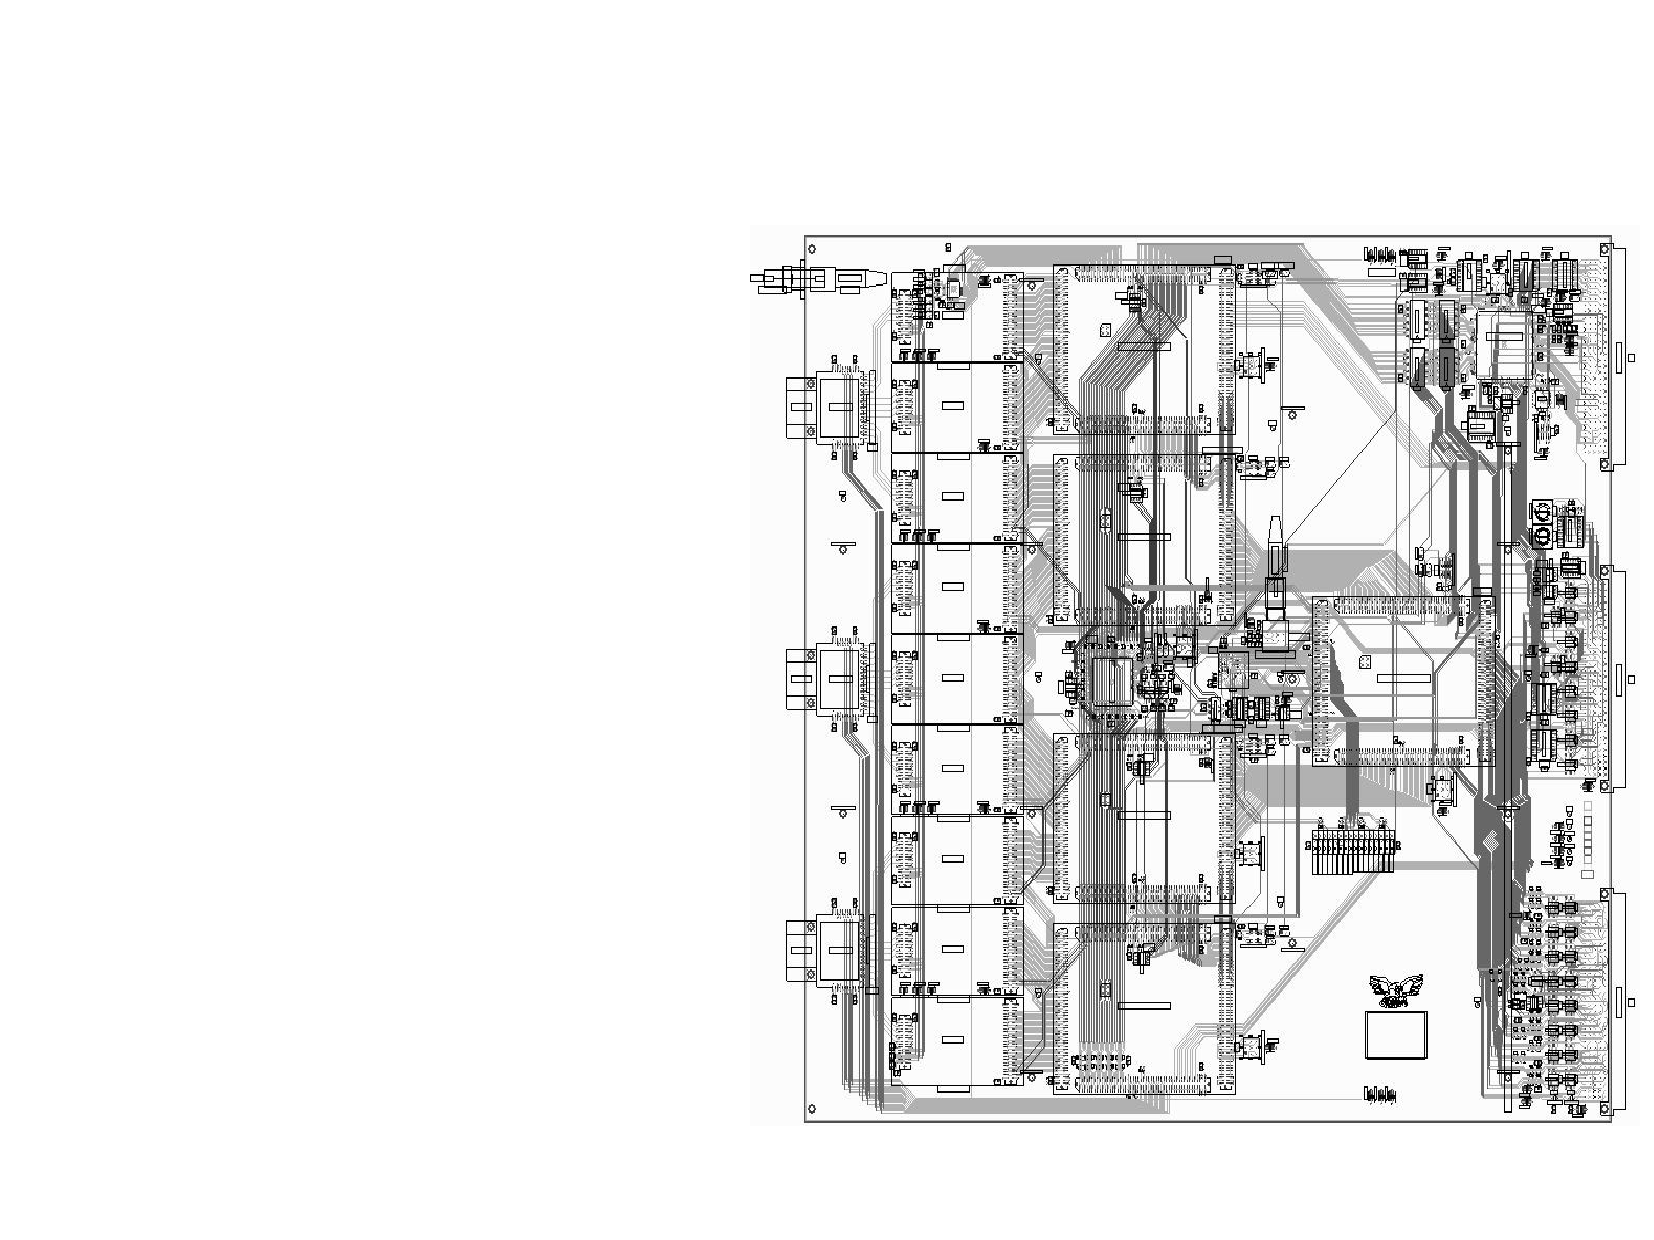
\includegraphics[width=0.45\textwidth]{pFED.pdf}
\end{center}
\caption{A schematic of the pixel FED.}
\label{fig:pFED}
\end{figure}

\clearpage

\subsubsection{The Pixel FEC}

The Pixel Front End Controller (FEC) sends triggers, clocks 
and programming data to the ROCs. For the pixel detector, 
we use a one-way `fast' I2C protocol to send this data.
We need to send 1 byte of data per pixel, or 66 MB of data
for the entire detector. For this, we use a 40 MHz serial line, 
and this calls for timing calibrations in order to enable downloads.

\begin{figure}[h]
\begin{center}
 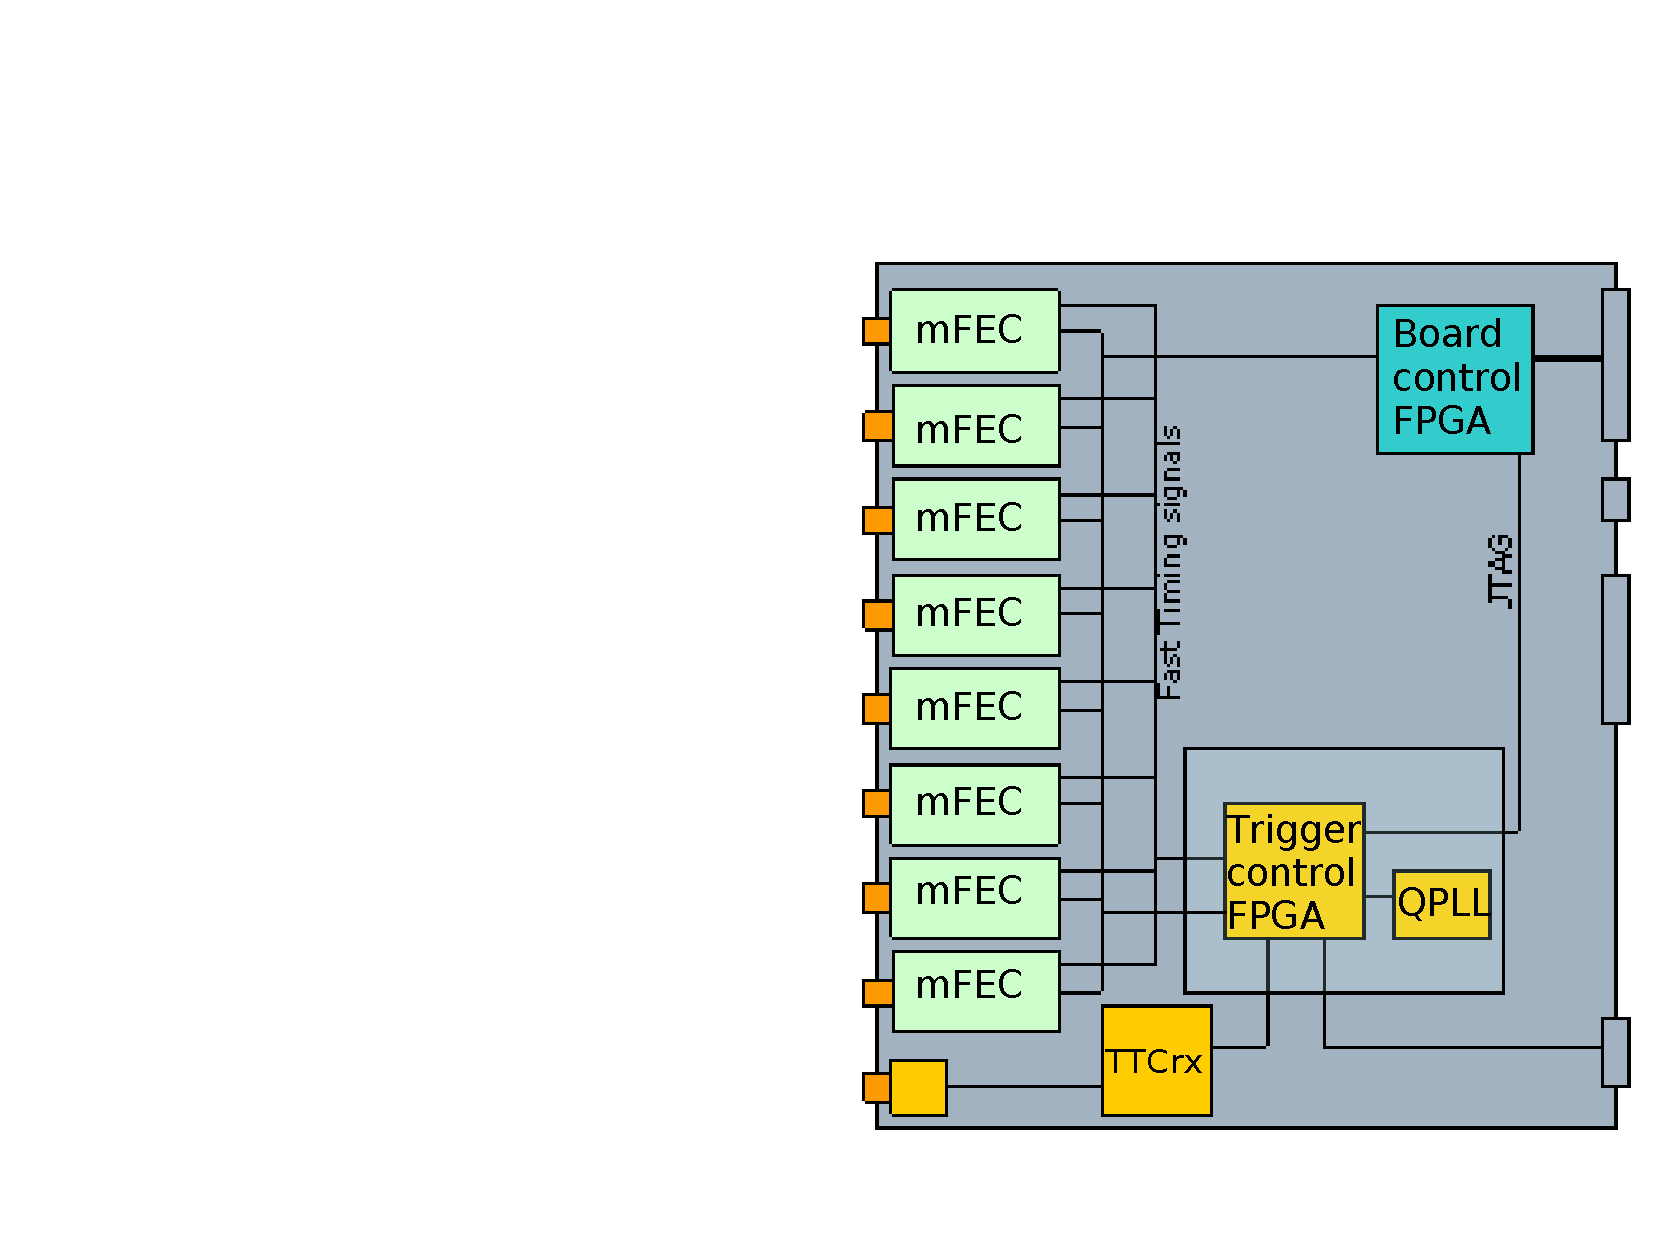
\includegraphics[width=0.45\textwidth]{pFEC.pdf}
\end{center}
\caption{A schematic of the pixel FEC.}
\label{fig:pFEC}
\end{figure}

\clearpage

\subsection{Installation at P5}

Table~\ref{tab:P5PCs} lists the online PCs that we have at P5
for pixel online software.

\begin{table}
\centering
\caption{Pixel online PCs at P5}
\label{tab:P5PCs}
\resizebox{\textwidth}{!}{
\begin{tabular}{lcccccccc}
\hline
\hline
Slot in rack & Node name     & Front & Label & Size & Function        & Comments     & OS \\ 
\hline
          -  & vmepcs2b18-17 & Pixel & -  & ?U      &  Histoviewer    &              & SLC4 \\
          19 & vmepcs2b18-16 & Pixel & 1/10  & 1U   &  VME/S1G01i     & BPix FECs    & SLC4 \\
          17 & vmepcs2b18-15 & Pixel & 10/10 & 1U   &  VME/S1G01e     & FPix FECs    & SLC4 \\
          16 & vmepcs2b18-14 & Pixel & 9/10  & 1U   &  VME/S1G04e     & BPix FEDs do & SLC4 \\
      14/15  & vmepcs2b18-13 & Pixel & 8/10  & 2U   &  VME/S1G04i     & BPix FEDs up & SLC4 \\
          13 & vmepcs2b18-12 & Pixel & 7/10  & 1U   &  VME/S1G03i     & FPix FEDs    & SLC4 \\
          12 & vmepcs2b18-11 & Pixel & 6/10  & 1U   &  PixelSuperFPix & FPix Supv.   & SLC4 \\
          11 & vmepcs2b18-10 & Pixel & 5/10  & 1U   &  PixelSuperBPix & BPix Supv.   & SLC4 \\
          10 & vmepcs2b18-09 & Pixel & 4/10  & 1U   &  DCS            & Fpix daq     & Win \\
           9 & vmepcs2b18-08 & Pixel & 3/10  & 1U   &  DCS/Siemens    &              & Win \\
           8 & vmepcs2b18-07 & Pixel & 2/10  & 1U   &  DCS/CAEN       &              & Win \\
             & vmepcs2b16-10 &       &       &      &  TTC+LTC Supv.  & TTC+LTC      & SLC4 \\
             &  cmsrc-pixel  &       &       &      &  L1 FM          & Pixel FM     & SLC4 \\
             &fmmpc-s1d12-08 &       &       &      &  FMM PC         & FMM PC       & SLC4 \\
             &  cmspsx       &       &       &      &  PSX server     & PSX server   & SLC4 \\
             &  srv-c2c02-05 &       &       &      &  DB server      &              & SLC4 \\
             &  srv-c2c02-06 &       &       &      &  DB server      &              & SLC4 \\
\hline
\hline
\end{tabular}
}
\end{table}

\begin{small}
\begin{table}
\centering
\caption{FED connections for FPIX}
\label{tab:FpixFED}
\resizebox{\textwidth}{!}{
\begin{tabular}{llcccclc}
\hline
\hline
Rack   & Crate   & Slot & VME addr.  & Channels & FED id & Name(Official) & Name(Construction) \\
\hline
S1G03  & upper   & 6    & 0x13000000 &  13-24   & 33     & BpO\_D(1,2)\_BLD(1,2,3)    & HC+Z1 1.1 2.1\\
S1G03  & upper   & 6    & 0x13000000 &  1-12    & 33     & BpO\_D(1,2)\_BLD(4,5,6)    & HC+Z1 1.2 2.2\\
S1G03  & upper   & 7    & 0x14000000 &  13-24   & 34     & Bp0\_D(1,2)\_BLD(7,8,9)    & HC+Z1 1.3 2.3\\
S1G03  & upper   & 7    & 0x14000000 &  1-12    & 34     & Bp0\_D(1,2)\_BLD(10,11,12) & HC+Z1 1.4 2.4\\
\hline
S1G03  & upper   & 5    & 0x12000000 &  1-12    & 32     & BpI\_D(1,2)\_BLD(1,2,3)    & HC+Z2 1.4 2.4\\
S1G03  & upper   & 5    & 0x12000000 &  13-24   & 32     & BpI\_D(1,2)\_BLD(4,5,6)    & HC+Z2 1.3 2.3\\
S1G03  & upper   & 8    & 0x15000000 &  1-12    & 35     & BpI\_D(1,2)\_BLD(7,8,9)    & HC+Z2 1.2 2.2\\
S1G03  & upper   & 8    & 0x15000000 &  13-24   & 35     & BpI\_D(1,2)\_BLD(10,11,12) & HC+Z2 1.1 2.1\\
\hline
S1G03  & upper   & 11   & 0x17000000 &  13-24   & 37     & BmI\_D(1,2)\_BLD(1,2,3)    & HC-Z1 1.1 2.1\\
S1G03  & upper   & 11   & 0x17000000 &  1-12    & 37     & BmI\_D(1,2)\_BLD(4,5,6)    & HC-Z1 1.2 2.2\\
S1G03  & upper   & 12   & 0x18000000 &  13-24   & 38     & BmI\_D(1,2)\_BLD(7,8,9)    & HC-Z1 1.3 2.3\\
S1G03  & upper   & 12   & 0x18000000 &  1-12    & 38     & BmI\_D(1,2)\_BLD(10,11,12) & HC-Z1 1.4 2.4\\
\hline
S1G03  & upper   & 10   & 0x16000000 &  1-12    & 36     & BmO\_D(1,2)\_BLD(1,2,3)    & HC-Z2 1.4 2.4\\
S1G03  & upper   & 10   & 0x16000000 &  13-24   & 36     & BmO\_D(1,2)\_BLD(4,5,6)    & HC-Z2 1.3 2.3\\
S1G03  & upper   & 13   & 0x19000000 &  1-12    & 39     & BmO\_D(1,2)\_BLD(7,8,9)    & HC-Z2 1.2 2.2\\
S1G03  & upper   & 13   & 0x19000000 &  13-24   & 39     & BmO\_D(1,2)\_BLD(10,11,12) & HC-Z2 1.1 2.1\\
\hline
\hline
\end{tabular}
}
\end{table}
\end{small}

\begin{small}
\begin{table}
\centering
\caption{FEC connections for FPIX}
\label{tab:FpixFEC}
\resizebox{\textwidth}{!}{
\begin{tabular}{llllclc}
\hline
\hline
Rack   & Crate   & Slot & VME addr. & mFEC & Name(Official) & Name(Construction) \\
\hline
S1G01  & middle  & 5    & 0x28000000 & 3    & BpO\_D(1,2)\_BLD(1,2,3)    & HC+Z1 1.1 2.1\\
S1G01  & middle  & 5    & 0x28000000 & 4    & BpO\_D(1,2)\_BLD(4,5,6)    & HC+Z1 1.2 2.2\\
S1G01  & middle  & 5    & 0x28000000 & 5    & Bp0\_D(1,2)\_BLD(7,8,9)    & HC+Z1 1.3 2.3\\
S1G01  & middle  & 5    & 0x28000000 & 6    & Bp0\_D(1,2)\_BLD(10,11,12) & HC+Z1 1.4 2.4\\
\hline
S1G01  & middle  & 5    & 0x28000000 & 8    & BpI\_D(1,2)\_BLD(1,2,3)    & HC+Z2 1.4 2.4\\
S1G01  & middle  & 5    & 0x28000000 & 7    & BpI\_D(1,2)\_BLD(4,5,6)    & HC+Z2 1.3 2.3\\
S1G01  & middle  & 5    & 0x28000000 & 2    & BpI\_D(1,2)\_BLD(7,8,9)    & HC+Z2 1.2 2.2\\
S1G01  & middle  & 5    & 0x28000000 & 1    & BpI\_D(1,2)\_BLD(10,11,12) & HC+Z2 1.1 2.1\\
\hline
S1G01  & middle  & 10   & 0x50000000 & 3    & BmI\_D(1,2)\_BLD(1,2,3)    & HC-Z1 1.1 2.1\\
S1G01  & middle  & 10   & 0x50000000 & 4    & BmI\_D(1,2)\_BLD(4,5,6)    & HC-Z1 1.2 2.2\\
S1G01  & middle  & 10   & 0x50000000 & 5    & BmI\_D(1,2)\_BLD(7,8,9)    & HC-Z1 1.3 2.3\\
S1G01  & middle  & 10   & 0x50000000 & 6    & BmI\_D(1,2)\_BLD(10,11,12) & HC-Z1 1.4 2.4\\
\hline
S1G01  & middle  & 10   & 0x50000000 & 8    & BmO\_D(1,2)\_BLD(1,2,3)    & HC-Z2 1.4 2.4\\
S1G01  & middle  & 10   & 0x50000000 & 7    & BmO\_D(1,2)\_BLD(4,5,6)    & HC-Z2 1.3 2.3\\
S1G01  & middle  & 10   & 0x50000000 & 2    & BmO\_D(1,2)\_BLD(7,8,9)    & HC-Z2 1.2 2.2\\
S1G01  & middle  & 10   & 0x50000000 & 1    & BmO\_D(1,2)\_BLD(10,11,12) & HC-Z2 1.1 2.1\\
\hline
\hline
\end{tabular}
}
\end{table}
\end{small}

\begin{small}
\begin{table}
\centering
\caption{CCU connections for FPIX}
\label{tab:FpixCCU}
\begin{tabular}{llcccc}
\hline
\hline
Rack   & Crate   & Slot & mFEC & Name(Official) & Name(Construction) \\
\hline
S1G01  &  middle & 18   &  8   & BpI            & HC+Z2 \\
S1G01  &  middle & 18   &  7   & BpO            & HC+Z1 \\
S1G01  &  middle & 18   &  6   & Bm0            & HC-Z2 \\
S1G01  &  middle & 18   &  5   & BmI            & HC-Z1 \\
\hline
\hline
\end{tabular}
\end{table}
\end{small}


